\setlength{\headheight}{14.49998pt}

\chapter{Example01}\label{chapter:Capitolo1}
In questo primo capitolo tratterò del primo esempio che ci è stato mostrato nel corso di Ingegneria del software: scriveremo in una classe 2 metodi (Waiter, Notifier) attraverso una labda-expression, che gestiranno al loro interno dei Thread e svolgeranno operazioni rispettivamente di wait() e notify().
%
\newline
\newline
%
Innanzitutto è necessario fare una doverosa precisazione sullo stato e metodi dei Threads (Figura~\ref{fig:one}).
\begin{figure}[ht]
	\centering
	\begin{subfigure}{0.5\textwidth}
		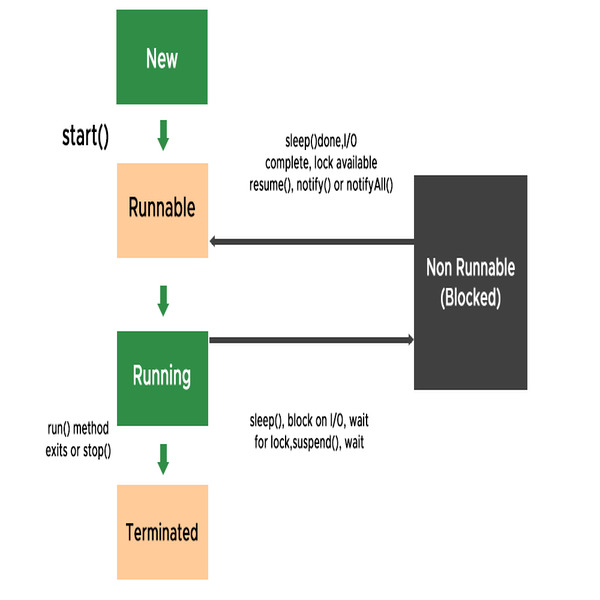
\includegraphics[width=1.0\textwidth]{Immagini/image_thread1.jpg}
		\caption{Stato del Thread}
	\end{subfigure}%
	\begin{subfigure}{0.5\textwidth}
		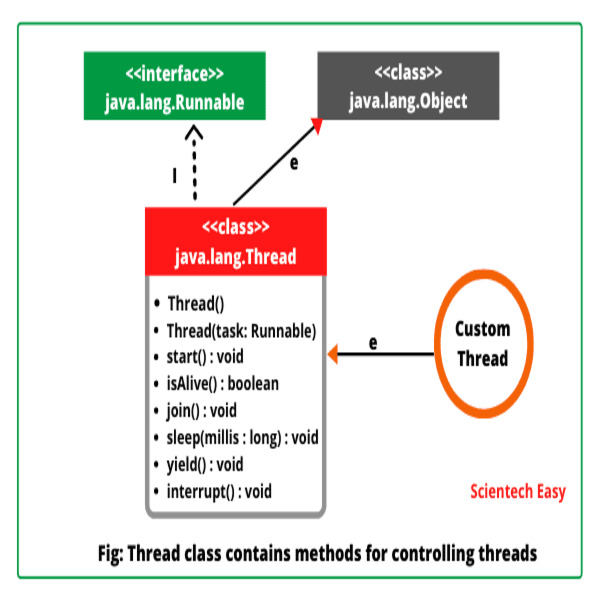
\includegraphics[width=1.0\textwidth]{Immagini/image_thread2.jpg}
		\caption{Metodi del Thread}
	\end{subfigure}
	\caption{Stati e Metodi del Thread}
	\label{fig:one}
\end{figure}
%
\newline
%
Attraverso la seguente tabella è possibile per metodo, ottenere una breve descrizione. 
\newline
\begin{table}[ht]
\centering
	\resizebox{0.99\linewidth}{!}{
            \begin{tabular}{|c|c|}
                \hline
                \rowcolor[HTML]{CBCEFB} 
                {\color[HTML]{333333} \textbf{Metodo}} & {\color[HTML]{333333} \textbf{Significato}} \\ \hline
                {\color[HTML]{9A0000} \textbf{getName}} & \textit{ottiene il nome del Thread} \\ \hline
                {\color[HTML]{9A0000} \textbf{getPriority}} & \textit{ottiene la priorità del Thread} \\ \hline
                {\color[HTML]{9A0000} \textbf{isAlive}} & \textit{determina se il Thread è ancora in esecuzione} \\ \hline
                {\color[HTML]{9A0000} \textbf{join}} & \textit{attende che il Thread termini} \\ \hline
                {\color[HTML]{9A0000} \textbf{run}} & \textit{mette in esecuzione il Thread} \\ \hline
                {\color[HTML]{9A0000} \textbf{sleep}} & \textit{sospende il thread per un periodo di tempo} \\ \hline
                {\color[HTML]{9A0000} \textbf{start}} & \textit{attiva il thread attraverso il metodo ``run"} \\ \hline
            \end{tabular}
        }
        \vspace*{2mm}
	\caption{Descrizione Metodi}
	\label{tab:perf}
\end{table}
%
\newline
Abbiamo precedente visto la costruzione dei thread in JAVA (estendendo Thread o implementando
Runnable) e abbiamo visto come costruire un progetto in Eclipse. Abbiamo visto come
aggiungere una classe in un package, quindi usiamo quello appena imparato per crearne due:
\begin{itemize}
    \item un thread \emph{\textbf{Waiter}} rimane in attesa aspettando la notifica di un altro;
    \item un thread \emph{\textbf{Notifier}} dopo un'attesa di tot secondi randomica, notifica con \functionStyle{notifyAll()}.
\end{itemize}


\section{Costruzione dei thread}
\subsection{Notifier}
Al suo interno estendiamo la classe \objectStyle{Thread}, siccome uno dei due modi per creare thread è o
questo, o implementare l'interfaccia Runnable. Siccome il metodo \functionStyle{run()} (seppure vuoto) esiste
già all'interno di \objectStyle{Thread}, facciamo \functionStyle{@Override} per scriverne un'implementazione.
%
\newline
\newline
%
Inoltre dobbiamo catturare l'eccezione perché quando siamo in stato d'attesa qualcuno dall'esterno, può bloccare il \objectStyle{Thread} che lancerà, per ciascuno, \emph{InterruptedException}.
Ogni \objectStyle{Thread} verrà interrotto
%
\newline
\newline
%
Se il Waiter deve fare \functionStyle{wait()} su un oggetto, e il Notifier deve fare \functionStyle{notifyAll()} su un
oggetto, quello sarà lo stesso oggetto, che è \objectStyle{Example01}.
Notifier non vede tuttavia l'oggetto \objectStyle{Example01}. 
Ragionevolmente lo scopo di Notifier è solo quello di costruire un thread e fare \functionStyle{notifyAll()},
mentre quello del Waiter e' fare \functionStyle{wait()}.
Un nuovo file separato dall'oggetto \objectStyle{Example01} non ha molto senso, siccome entrambi Notifier
e Waiter devono vedersi gli stati a vicenda.
Spostiamo quindi il codice della Notifier dentro a \objectStyle{Example01}, cancellando il vecchio file e
mentre lo facciamo, anonimizziamo la classe siccome dargli un nome non e' necessario, siccome
la usiamo una volta soltanto.

\subsection{Waiter}
Si dovrà mettere in attesa e aspettare che il Notifier lo notifichi.
Per crearlo, ci basta prima ridefinire l'implementazione di \interfaceStyle{Runnable}. \\
L'oggetto su cui facciamo operazioni e' uno di tipo \objectStyle{Object}, privato ad \objectStyle{Example01}, e lo scriviamo
in cima, prima della \functionStyle{go()}. Chiamiamo per semplicita' questo oggetto: \textbf{\emph{mutex}}.
%
\newline
\newline
%
Abbiamo tuttavia un problema, non irrilevante, di sincronizzazione. 
Seguiamo questo ragionamento per identificarlo (vedi commenti in alto numerati):
\begin{enumerate}
    \item facciamo start() di Notifier;
    \item facciamo sleep(5000);
    \item facciamo notifyAll();
    \item facciamo start() del Waiter;
    \item facciamo System.out.println(``Waiter started");
    \item facciamo wait();
\end{enumerate}

Niente ci garantisce che la \functionStyle{NotifyAll()} venga fatta dopo la \functionStyle{wait()}. 
Potrebbe succedere, anche se poco probabile nel caso di 5 secondi di attesa, che i due thread
partano ma senza l'ordine da noi voluto. 

\section{Example01 Programma}
Figura~\ref{fig:two} mostra l'output del programma.

\subsection{Example01.java}
\begin{algorithm}[ht]
	\caption{Example01.java}
	\label{lst:genic_mpi}
	\begin{lstlisting}
    package it.unipr.informatica.example; 
    public class Example01 { 
        private Object mutex = new Object(); 
        private boolean waitInProgress = false; 
     
         public void go() { 
            waitInProgress = false; 
            Thread notifier = new Thread(this::doNotify); 
            Thread notifier = new Thread(this::doWait); 
            notifier.start(); 
            waiter.start(); 
         }   
         private void doWait() { 
             System.out.println("Waiter started"); 
             synchronized(mutex) { 
                 waitInProgress = true;
                 mutex.notifyAll();  
                 try { 
                    mutex.wait(); 
                 } catch(Throwable throwable) { //blank } 
             } 
             System.out.println("Waiter terminated"); 
         }  
         private void doNotify() { 
             System.out.println("Notifier started"); 
             synchronized(mutex) { 
                 try { 
                    while (!waitInProgress)  mutex.wait();  
                    Thread.sleep(5000); 
                    mutex.notifyAll(); 
                 } catch (Throwable trhowable) { //blank } 
             } 
             System.out.println("Notifier terminated");
         } 
         public static void main(String[] args) { 
             new Example01().go(); 
         } 
    } 
	\end{lstlisting}
\end{algorithm}

\subsection{Output Programma}{Example01.java}
\begin{figure}[ht]
	\centering
	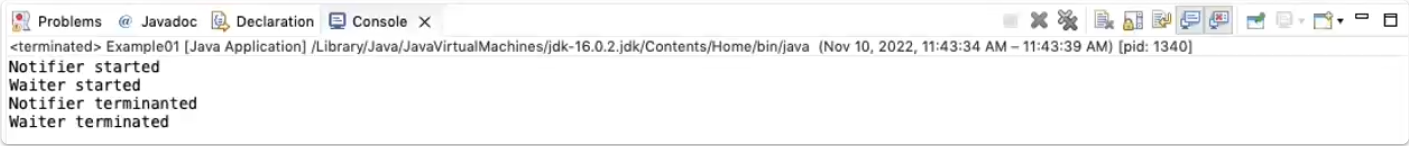
\includegraphics[width=1.0\textwidth]{Immagini/output_code1.png}
	\caption{Output del Programma (Example01.java)}
	\label{fig:two}
\end{figure}


\section{Citazioni}
La scrittura di questo report accademico è stato possibile anche grazie a testi che ci sono stati assegnati durante il corso
come:  \cite{lewis2009component,robles2004software}.
Estremamante importante è stato anche l'articolo del professore Lars Bendix \cite{bendixshort}, che oltretutto, è stato mio insegnante all'università per 2 settimane.